\documentclass[11pt]{article}

\usepackage[margin=1in]{geometry}
\usepackage{graphicx}
\usepackage{booktabs}
\usepackage{longtable}
\usepackage{array}
\usepackage[strings]{underscore}
\usepackage{hyperref}
\usepackage{xcolor}
\usepackage{amssymb}
\usepackage{enumitem}
\usepackage{float}

\hypersetup{
  colorlinks=true,
  linkcolor=blue,
  urlcolor=blue,
  citecolor=blue
}

\setlist[itemize]{leftmargin=1.5em}

\newcommand{\code}[1]{\texttt{#1}}
\newcommand{\checked}{\texttt{[x]}}
\newcommand{\unchecked}{\texttt{[ ]}}

\title{DDM501 Final Project Report\\Real-Time Fraud Detection ML System}
\author{Repository: \code{Final_Project_DMM501_Group1}}
\date{Generated from repository implementation (as of 2026-04-14)}

\begin{document}
\maketitle
\tableofcontents
\newpage

% --------------------------------------------------
\section*{SECTION 1 — Problem Definition \& Requirements}
\addcontentsline{toc}{section}{SECTION 1 — Problem Definition \& Requirements}

\subsection*{1.1 Problem statement}
Build an end-to-end ML system that scores credit-card transactions for fraud risk in near real time. The system must (1) train and benchmark models on the Kaggle Credit Card Fraud dataset, (2) serve predictions via an API, (3) provide a demo UI for live scoring, and (4) expose monitoring and alerting to support operational visibility.

\subsection*{1.2 Business context}
Fraud scoring is used to reduce financial loss and operational cost by prioritizing transactions for review or intervention. In this project, the fraud score is treated as a decision-support signal with an explicit threshold policy (stored as model metadata and returned by the API).

\subsection*{1.3 Dataset description (Kaggle fraud dataset)}
\textbf{Dataset used in this repository:} \code{data/archive/creditcard.csv}. The pipeline validates the schema and records it to \code{artifacts/reports/dataset_schema.json}.

\begin{itemize}
  \item Rows/columns: 284{,}807 rows and 31 columns (\code{Time}, \code{V1..V28}, \code{Amount}, \code{Class}). See \code{artifacts/reports/dataset_schema.json}.
  \item Target: \code{Class} (0 = non-fraud, 1 = fraud).
  \item Feature contract used end-to-end (30 floats): \code{[Time, V1..V28, Amount]}. Stored in \code{artifacts/models/model_info.json} and enforced by the API.
\end{itemize}

\subsection*{1.4 Key challenges}
\begin{itemize}
  \item \textbf{Extreme class imbalance:} 492 fraud cases out of 284{,}807 total (\(\approx 0.1727\%\)). See \code{artifacts/reports/class_distribution.json}.
  \item \textbf{Accuracy is misleading:} A classifier can achieve \(\approx 99.9\%\) accuracy while performing poorly on the fraud class; this repo prioritizes PR-AUC and threshold-tuned precision/recall.
  \item \textbf{Real-time serving constraints:} predictions must be fast, stable, and observable (latency and error rate monitored).
  \item \textbf{Operational policy:} threshold selection is a business decision (trade-off between false positives and false negatives) and must be explicit and versioned.
\end{itemize}

\subsection*{1.5 Success metrics (actual metrics and targets)}
\textbf{Note:} Model results below are taken from generated artifacts in \code{artifacts/} (not fabricated). The benchmark workflow is implemented in \code{src/pipelines/run_model_workflow.py}.

\paragraph{Model metrics (from tuned test split)}
From \code{artifacts/reports/model_selection_summary.json}:
\begin{itemize}
  \item \textbf{Baseline (Logistic Regression, tuned threshold 0.99):}
    PR-AUC=0.7929, ROC-AUC=0.9680, Precision=0.6742, Recall=0.8108, F1=0.7362.
  \item \textbf{Improved (LightGBM, tuned threshold 0.84):}
    PR-AUC=0.7161, ROC-AUC=0.8828, Precision=0.8852, Recall=0.7297, F1=0.8000.
  \item \textbf{Selected deployable model (by PR-AUC rule):} \emph{Logistic Regression} (selected because improved PR-AUC \(<\) baseline PR-AUC). See \code{artifacts/models/model_info.json}.
\end{itemize}

\paragraph{System metrics (monitored)}
Implemented as Prometheus metrics in \code{src/monitoring/metrics.py}, exposed at \code{GET /metrics} by \code{src/api/main.py}:
\begin{itemize}
  \item Request volume: \code{api\_requests\_total\{endpoint,method,http\_status\}}
  \item Latency histogram: \code{api\_request\_latency\_seconds\_bucket\{endpoint,method,...\}}
  \item Prediction counts: \code{fraud\_predictions\_total\{label\}}
  \item Score aggregation: \code{fraud\_scores\_sum\_total} and \code{fraud\_scores\_count\_total}
\end{itemize}

\paragraph{Business metrics (demo-grade)}
This project treats PR-AUC as a proxy for review efficiency and uses threshold-tuned precision/recall to represent operational trade-offs (e.g., controlling false-positive review load while maintaining fraud recall).

\subsection*{1.6 Functional requirements (from implementation)}
Aligned with \code{README.md} and verified in code:
\begin{itemize}
  \item \textbf{F1:} \code{POST /predict} returns \code{fraud\_probability} and threshold-based \code{fraud\_label}. (\code{src/api/main.py})
  \item \textbf{F2:} \code{GET /health} returns \code{model\_loaded}, \code{model\_version}, \code{expected\_features}, \code{threshold}. (\code{src/api/main.py})
  \item \textbf{F3:} \code{GET /metrics} exposes Prometheus metrics. (\code{src/api/main.py}, \code{src/monitoring/metrics.py})
  \item \textbf{F4:} Training/benchmark workflow produces model artifacts + reports. (\code{src/pipelines/run\_model\_workflow.py})
  \item \textbf{F5:} \code{GET /dataset/samples} returns dataset-backed samples for demo/verification. (\code{src/api/main.py}, \code{src/data/samples.py})
  \item \textbf{F6:} Demo UI performs live scoring against backend \code{/predict}. (\code{frontend/})
  \item \textbf{F7:} Observability stack configs: Prometheus + Grafana + alert rules via Docker Compose. (\code{deployment/})
\end{itemize}

\subsection*{1.7 Non-functional requirements (from implementation)}
\begin{itemize}
  \item \textbf{Latency visibility and alerting:} Prometheus rule \code{FraudApiHighP95Latency} alerts if p95 \(> 0.5s\) for 10m. (\code{deployment/prometheus/alerts.yml})
  \item \textbf{Reliability visibility:} Prometheus rule \code{FraudApiHigh5xxErrorRate} alerts if 5xx \(> 5\%\). (\code{deployment/prometheus/alerts.yml})
  \item \textbf{Reproducibility:} benchmark script writes deterministic split info and saves artifacts under \code{artifacts/}. (\code{artifacts/reports/split\_info.json})
  \item \textbf{CI quality gate:} GitHub Actions runs tests with coverage threshold \(\ge 80\%\). (\code{.github/workflows/ci.yml})
  \item \textbf{Containerized deployment:} API + frontend + MLflow + Prometheus + Grafana in Compose with healthchecks. (\code{deployment/docker-compose.yml})
\end{itemize}

% --------------------------------------------------
\section*{SECTION 2 — System Design \& Architecture}
\addcontentsline{toc}{section}{SECTION 2 — System Design \& Architecture}

\subsection*{2.1 High-level architecture (implemented)}
Architecture is documented in \code{ARCHITECTURE.md} and implemented across \code{src/}, \code{frontend/}, and \code{deployment/}.

\begin{itemize}
  \item \textbf{Training/Benchmarking:} \code{python -m src.pipelines.run\_model\_workflow} produces artifacts in \code{artifacts/}.
  \item \textbf{Model serving API:} FastAPI app in \code{src/api/main.py} loads \code{artifacts/models/final\_model.joblib}.
  \item \textbf{Frontend demo:} static dashboard in \code{frontend/} streams transactions and calls \code{/predict}.
  \item \textbf{Monitoring:} Prometheus scrapes \code{/metrics}; Grafana dashboard auto-provisioned.
  \item \textbf{Experiment tracking:} MLflow SQLite backend at \code{artifacts/mlflow.db} (and Compose MLflow server).
\end{itemize}

\subsection*{2.2 Component breakdown}
\paragraph{ML pipeline}
\begin{itemize}
  \item \code{src/pipelines/run\_model\_workflow.py}: end-to-end dataset validation, EDA, baseline vs improved model training, threshold tuning, SHAP, selection, and artifact export.
  \item \code{src/pipelines/train\_pipeline.py}: smaller training pipeline (supports synthetic fallback; optional LightGBM if available).
\end{itemize}

\paragraph{API}
\begin{itemize}
  \item FastAPI endpoints in \code{src/api/main.py} with typed schemas in \code{src/api/schemas.py}.
  \item Model loading via \code{src/models/loader.py} using \code{MODEL\_PATH} + metadata \code{model\_info.json}.
\end{itemize}

\paragraph{Frontend}
\begin{itemize}
  \item Vanilla JS dashboard: \code{frontend/index.html}, \code{frontend/app.js}, \code{frontend/ui.js}.
  \item Streams transactions (real samples from \code{frontend/real-samples.json} or random generation) and scores them via \code{/predict}.
\end{itemize}

\paragraph{Monitoring}
\begin{itemize}
  \item Prometheus config: \code{deployment/prometheus/prometheus.yml} (scrape interval 5s).
  \item Alert rules: \code{deployment/prometheus/alerts.yml}.
  \item Grafana dashboard: \code{deployment/grafana/dashboards/fraud\_api.json}.
\end{itemize}

\subsection*{2.3 Data flow (actual implementation)}
\begin{itemize}
  \item \textbf{Training:} \code{data/archive/creditcard.csv} \(\rightarrow\) split (70/15/15) \(\rightarrow\) baseline + LightGBM tuning \(\rightarrow\) threshold sweep on validation \(\rightarrow\) test evaluation \(\rightarrow\) artifacts in \code{artifacts/}.
  \item \textbf{Inference:} frontend feature vector (30 floats) \(\rightarrow\) \code{POST /predict} \(\rightarrow\) \code{predict\_proba} \(\rightarrow\) label by stored threshold \(\rightarrow\) UI + Prometheus metrics updated.
  \item \textbf{Observability:} \code{/metrics} scraped by Prometheus \(\rightarrow\) Grafana panels + Prometheus alert evaluation.
\end{itemize}

\subsection*{2.4 Technology stack (from \code{requirements.txt} and deployment)}
\begin{itemize}
  \item ML: NumPy, Pandas, scikit-learn, LightGBM, SHAP, Matplotlib, Joblib
  \item Serving: FastAPI, Uvicorn, Pydantic
  \item Tracking: MLflow (SQLite backend in \code{artifacts/mlflow.db})
  \item Monitoring: prometheus-client, Prometheus, Grafana
  \item Deployment: Docker, Docker Compose
  \item Frontend: HTML/CSS + vanilla JavaScript
\end{itemize}

\subsection*{2.5 Trade-offs (as implemented)}
\begin{itemize}
  \item \textbf{Accuracy vs. latency:} Simple tabular models (LogReg/LightGBM) keep inference fast and predictable; no deep model introduced.
  \item \textbf{Precision vs. recall:} Threshold tuning explicitly selects an operating point; the chosen threshold is stored in \code{artifacts/models/model\_info.json}.
  \item \textbf{Model selection criterion:} This repo selects the deployable model primarily by \textbf{test PR-AUC} comparison between baseline and improved (see \code{src/pipelines/run\_model\_workflow.py}).
  \item \textbf{Demo realism:} Frontend simulates streaming with a loop and real dataset samples rather than integrating a message queue (Kafka/Kinesis not implemented).
\end{itemize}

% --------------------------------------------------
\section*{SECTION 3 — Implementation}
\addcontentsline{toc}{section}{SECTION 3 — Implementation}

\subsection*{A. ML Pipeline}

\subsubsection*{A1. Dataset usage}
\begin{itemize}
  \item Primary dataset path: \code{data/archive/creditcard.csv} (validated in \code{artifacts/reports/dataset\_schema.json}).
  \item Feature columns used: 30 features \code{Time}, \code{V1..V28}, \code{Amount} (stored in \code{artifacts/models/model\_info.json}).
  \item Split: train=199{,}364, val=42{,}721, test=42{,}722 with seed=42 (see \code{artifacts/reports/split\_info.json}).
\end{itemize}

\subsubsection*{A2. Preprocessing}
\begin{itemize}
  \item API-side preprocessing is shape/typing only: \code{src/features/preprocess.py} converts list \(\rightarrow\) \code{numpy.ndarray} of shape \((1,n)\).
  \item Baseline model uses a scikit-learn \code{Pipeline(StandardScaler, LogisticRegression)}; scaling is part of the artifact (see \code{src/pipelines/run\_model\_workflow.py}).
  \item Improved LightGBM uses raw numeric features; preprocessing recorded as identity in \code{artifacts/models/final\_preprocessing\_identity.json}.
\end{itemize}

\subsubsection*{A3. Models (baseline + improved)}
\begin{itemize}
  \item \textbf{Baseline:} Logistic Regression with \code{class\_weight="balanced"} and \code{StandardScaler}. Artifact: \code{artifacts/models/baseline\_logistic\_regression\_pipeline.joblib}.
  \item \textbf{Improved:} LightGBM (\code{LGBMClassifier}) tuned by validation PR-AUC across a small \code{ParameterGrid}. Artifact: \code{artifacts/models/improved\_lightgbm.joblib}. Tuning log: \code{artifacts/benchmarks/improved\_hyperparameter\_tuning.csv}.
  \item \textbf{Final deployable:} Selected model exported to \code{artifacts/models/final\_model.joblib} plus metadata \code{artifacts/models/model\_info.json}.
\end{itemize}

\subsubsection*{A4. Evaluation metrics}
Evaluation is implemented in \code{src/pipelines/run\_model\_workflow.py} and exported to artifacts:
\begin{itemize}
  \item Confusion matrices: \code{artifacts/figures/confusion\_matrix.png} (baseline) and \code{artifacts/figures/improved\_confusion\_matrix.png}.
  \item ROC/PR curves: \code{artifacts/figures/baseline\_roc\_curve.png}, \code{artifacts/figures/baseline\_pr\_curve.png}, \code{artifacts/figures/improved\_roc\_curve.png}, \code{artifacts/figures/improved\_pr\_curve.png}.
  \item Classification reports: \code{artifacts/reports/baseline\_classification\_report.json} and \code{artifacts/reports/improved\_classification\_report.json}.
\end{itemize}

\subsubsection*{A5. Threshold tuning}
\begin{itemize}
  \item Threshold sweep is computed on validation scores (\code{_threshold\_sweep}) and the best threshold is chosen by max F1 (\code{_best\_threshold\_from\_f1}).
  \item Threshold curves exported:
    \code{artifacts/benchmarks/baseline\_threshold\_tuning.csv} and \code{artifacts/benchmarks/improved\_threshold\_tuning.csv}.
  \item Tuned thresholds (from \code{artifacts/reports/model\_selection\_summary.json}):
    baseline=0.99, improved=0.84.
\end{itemize}

\subsubsection*{A6. Artifact outputs (actual files)}
\begin{itemize}
  \item Deployable model: \code{artifacts/models/final\_model.joblib}
  \item Deploy metadata: \code{artifacts/models/model\_info.json} (includes threshold, feature order, dataset path, metrics, selection timestamp)
  \item Benchmark summary: \code{artifacts/reports/benchmark\_summary.md}
  \item SHAP outputs: \code{artifacts/figures/shap\_summary.png}, \code{artifacts/benchmarks/shap\_importance\_table.csv}
\end{itemize}

\subsection*{B. Deployment}

\subsubsection*{B1. FastAPI backend}
Backend entrypoint: \code{src/api/main.py}. The Docker image is defined in \code{deployment/api/Dockerfile} and the Compose service \code{api} in \code{deployment/docker-compose.yml}.

\subsubsection*{B2. Model loading logic}
\begin{itemize}
  \item At startup, the API attempts to load a model via \code{src/models/loader.py}.
  \item Primary mode: \code{MODEL\_PATH} environment variable (Compose sets \code{/app/artifacts/models/final\_model.joblib}).
  \item Metadata: the loader reads \code{model\_info.json} next to the model artifact to obtain threshold, feature columns, dataset path, and selection timestamp.
  \item Safety: \code{/predict} returns HTTP 503 if model is not loaded; returns HTTP 422 for invalid feature length or non-finite values.
\end{itemize}

\subsubsection*{B3. API endpoints (actual contract)}
Implemented in \code{src/api/main.py} with schemas in \code{src/api/schemas.py}:
\begin{itemize}
  \item \textbf{\code{GET /health}}: status + model metadata (\code{model\_loaded}, \code{model\_version}, \code{expected\_features}, \code{threshold}, \code{model\_type}).
  \item \textbf{\code{POST /predict}}: request accepts \code{features: [float]} or \code{features\_by\_name: \{name: float\}}; response returns \code{fraud\_probability}, \code{fraud\_label}, threshold, version, request id.
  \item \textbf{\code{GET /metrics}}: Prometheus exposition format.
  \item \textbf{\code{GET /dataset/samples}}: samples from the recorded dataset path; supports \code{strategy=mixed|fraud|legit}.
\end{itemize}
Additional demo-support endpoints exist: \code{GET /features/schema} and \code{GET /features/random}.

\subsection*{C. Frontend}

\subsubsection*{C1. Real-time dashboard}
\begin{itemize}
  \item UI entry: \code{frontend/index.html} (Control Panel, Live Summary KPIs, Alert Panel, Chart, Live Transaction Feed).
  \item Logic: \code{frontend/app.js} orchestrates health polling and streaming scoring loop.
  \item Rendering: \code{frontend/ui.js} updates DOM, feed table, alert list, and chart canvas.
\end{itemize}

\subsubsection*{C2. Streaming logic (actual)}
\begin{itemize}
  \item Health poll every 5 seconds: \code{GET /health} to verify backend reachable and \code{expected\_features==30}.
  \item Stream loop: on Start, the UI repeatedly generates a transaction and calls \code{POST /predict} at an interval of 0.5s / 1s / 2s.
  \item Data sources:
    \begin{itemize}
      \item Real sample stream: dataset-backed sampling via \code{GET /dataset/samples} (production-like base rate, with rare fraud spikes for demo visibility).
      \item Random generated stream: synthetic feature vectors produced by \code{frontend/demo-data.js}.
    \end{itemize}
  \item Failure handling: stops stream after 4 consecutive errors (demo-friendly).
\end{itemize}

\subsubsection*{C3. Alert system and risk classification}
Implemented in \code{frontend/app.js}:
\begin{itemize}
  \item Risk tiers (policy-driven): \emph{LOW} if score \(< \) \code{threshold\_review}; \emph{REVIEW} if score is between \code{threshold\_review} and \code{threshold\_high}; \emph{HIGH} if score \( \ge \) \code{threshold\_high}.
  \item Alerts/cases are created for \emph{REVIEW} and \emph{HIGH} items and shown in the Alert Panel / Review queue.
\end{itemize}

\subsection*{D. Monitoring}

\subsubsection*{D1. Prometheus metrics}
Metrics are emitted in \code{src/monitoring/metrics.py} and exposed at \code{GET /metrics}.

\subsubsection*{D2. Grafana dashboards}
Dashboard definition: \code{deployment/grafana/dashboards/fraud\_api.json}. Panel titles include:
\begin{itemize}
  \item API Requests Per Second
  \item Request Latency (95th percentile)
  \item Average Risk Score
  \item Decisions by Tier
\end{itemize}

\subsubsection*{D3. Alert rules}
Alert rules are defined in \code{deployment/prometheus/alerts.yml} for:
\begin{itemize}
  \item High 5xx error rate (\(> 5\%\))
  \item High p95 latency (\(> 0.5s\))
  \item Prediction rate too low / too high
\end{itemize}

% --------------------------------------------------
\section*{SECTION 4 — Testing \& CI/CD}
\addcontentsline{toc}{section}{SECTION 4 — Testing \& CI/CD}

\subsection*{4.1 Test types (from \code{tests/})}
\begin{itemize}
  \item \textbf{Unit tests:} preprocessing and utility IDs (e.g., \code{tests/unit/test\_preprocess.py}, \code{tests/unit/test\_ids.py}).
  \item \textbf{Integration tests:} FastAPI endpoints with ASGI test client (e.g., \code{tests/integration/test\_api\_predict\_happy\_path.py}).
  \item \textbf{Data quality tests:} dataset loader behavior and target validity for synthetic data (\code{tests/data/test\_data\_quality\_placeholder.py}).
  \item \textbf{Model validation tests:} training produces artifacts; loaded model outputs probabilities in range (\code{tests/model/test\_model\_validation\_placeholder.py}).
\end{itemize}

\subsection*{4.2 Coverage strategy}
CI enforces a coverage threshold via \code{pytest-cov}:
\begin{itemize}
  \item Command: \code{pytest -q --cov=src --cov-report=term-missing --cov-fail-under=80}
  \item Workflow: \code{.github/workflows/ci.yml}
\end{itemize}

\subsection*{4.3 CI/CD pipeline (GitHub Actions)}
\begin{itemize}
  \item \textbf{CI:} installs dependencies, runs tests, fails if coverage \(< 80\%\). (\code{.github/workflows/ci.yml})
  \item \textbf{Docker validation:} builds API and frontend images; validates Compose file. (\code{.github/workflows/docker.yml})
\end{itemize}

\subsection*{4.4 What is verified vs not verified (this report)}
\begin{itemize}
  \item \textbf{Verified by repository evidence:} implementation exists; artifacts contain real benchmark outputs; API endpoints and monitoring configs are present.
  \item \textbf{Not re-executed in this report generation:} CI execution, Docker builds, and live Prometheus/Grafana runtime behavior are not run here; treat them as \emph{configured} and \emph{reproducible} rather than proved live in this session.
\end{itemize}

% --------------------------------------------------
\section*{SECTION 5 — Responsible AI}
\addcontentsline{toc}{section}{SECTION 5 — Responsible AI}

\subsection*{5.1 Explainability (SHAP)}
\begin{itemize}
  \item Implemented in \code{src/pipelines/run\_model\_workflow.py} for the LightGBM model.
  \item Outputs:
    \code{artifacts/figures/shap\_summary.png} and \code{artifacts/benchmarks/shap\_importance\_table.csv}.
\end{itemize}

\subsection*{5.2 Fairness limitations}
The dataset contains anonymized PCA components (\code{V1..V28}) and does not include protected attributes. As documented in \code{RESPONSIBLE\_AI.md}, demographic fairness metrics cannot be computed; fairness discussion is limited to proxy slices (e.g., amount/time buckets) and should be treated as insufficient evidence rather than proof.

\subsection*{5.3 Privacy considerations}
\begin{itemize}
  \item The API contract accepts numeric features only (\code{PredictRequest} in \code{src/api/schemas.py}).
  \item Recommended logging stance (documented in \code{RESPONSIBLE\_AI.md}): do not log raw feature vectors; log only request metadata and aggregated metrics.
\end{itemize}

\subsection*{5.4 Ethical risks and mitigations}
\begin{itemize}
  \item False positives: customer friction; mitigated via explicit threshold policy and a \emph{REVIEW} tier in the UI (human-in-the-loop workflow).
  \item False negatives: fraud loss; mitigated by tracking recall and documenting trade-offs.
  \item Over-trusting explanations: SHAP is not causal; documented limitations in \code{RESPONSIBLE\_AI.md}.
\end{itemize}

% --------------------------------------------------
\section*{SECTION 6 — Frontend Demo \& UI/UX}
\addcontentsline{toc}{section}{SECTION 6 — Frontend Demo \& UI/UX}

\subsection*{6.1 Dashboard layout (actual UI)}
From \code{frontend/index.html}:
\begin{itemize}
  \item Header: connection pill + model version + thresholds (review/high) + expected feature count.
  \item Control Panel: API Base URL, mode (real/random), speed, start/stop/reset.
  \item Live Summary KPIs: total processed, high risk (block), review queue, alert rate, avg risk score, last latency.
  \item Alert Panel: recent \emph{REVIEW} and \emph{HIGH} items.
  \item Chart: risk score over time with threshold overlays (review/high).
  \item Feed: append-only table with timestamp, request id, amount, score, tier, action, thresholds, latency, source.
\end{itemize}

\begin{figure}[H]
  \centering
  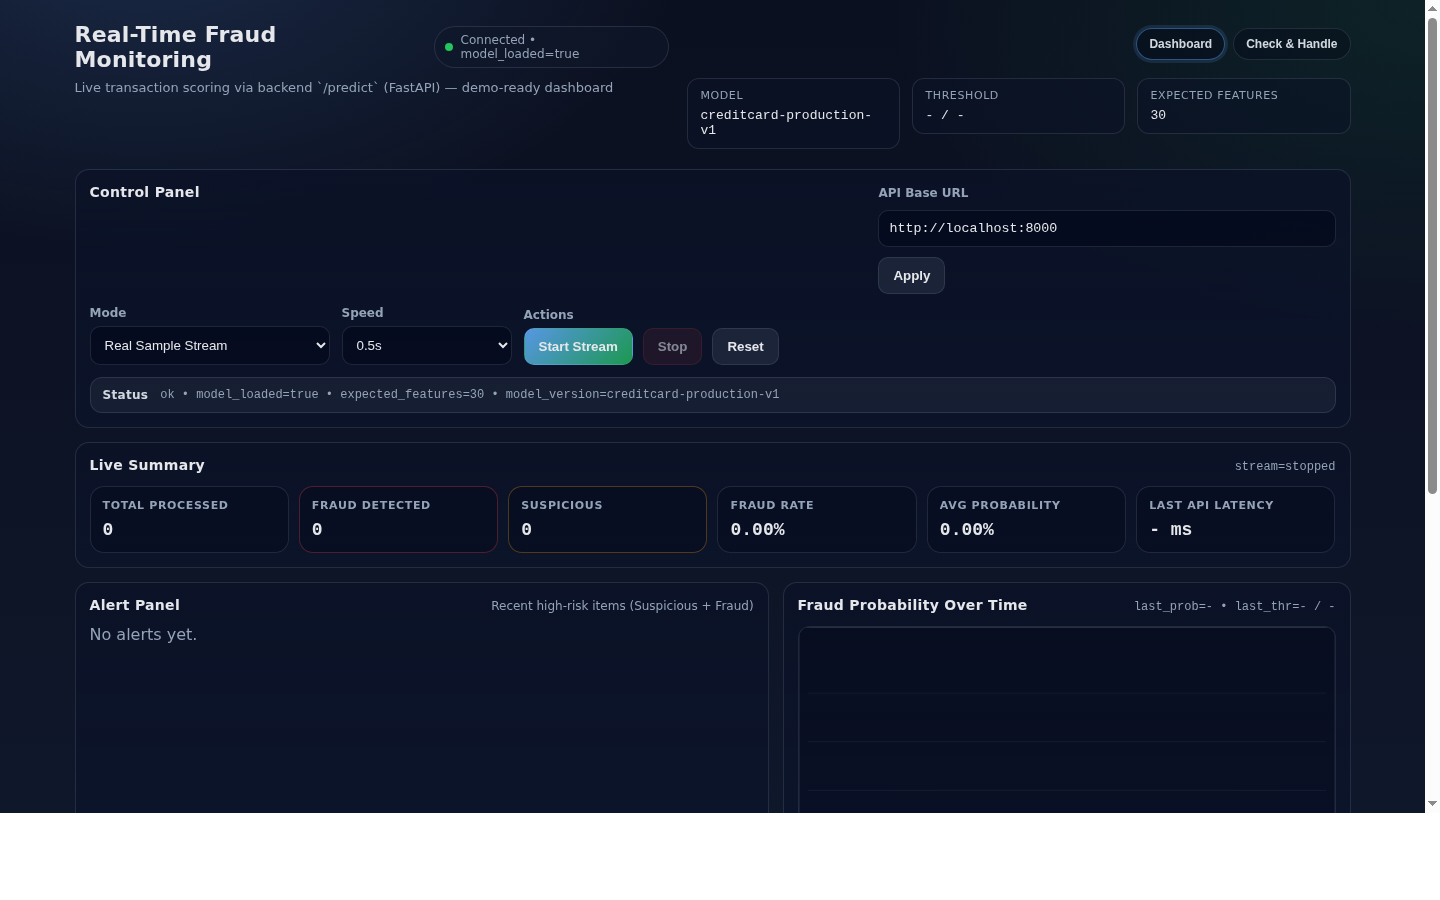
\includegraphics[width=0.95\linewidth]{../artifacts/figures/frontend_dashboard_live.png}
  \caption{Frontend dashboard screenshot (connected to backend). Source: \code{artifacts/figures/frontend_dashboard_live.png}.}
\end{figure}

\subsection*{6.2 Transaction monitoring and abnormal detection}
\begin{itemize}
  \item Every generated transaction triggers a backend \code{/predict} call; the UI uses the returned \code{risk\_score} as the primary signal.
  \item Risk tiering is policy-driven using backend thresholds (\code{threshold\_review}/\code{threshold\_high}) into LOW/REVIEW/HIGH.
  \item Alerts are UI-only (no external notification channel implemented).
\end{itemize}

\subsection*{6.3 Streaming demo}
Streaming is simulated (no Kafka/WebSockets). The demo intentionally keeps architecture simple:
\begin{itemize}
  \item A loop generates transactions (\code{frontend/demo-data.js}) and calls \code{/predict} at a fixed interval.
  \item The UI stops the stream after repeated errors to keep the live presentation stable.
\end{itemize}

% --------------------------------------------------
\section*{SECTION 7 — Dataset Explanation (IMPORTANT)}
\addcontentsline{toc}{section}{SECTION 7 — Dataset Explanation (IMPORTANT)}

\subsection*{7.1 Dataset structure}
From \code{artifacts/reports/dataset\_schema.json}:
\begin{itemize}
  \item 31 columns: \code{Time}, \code{V1..V28}, \code{Amount}, \code{Class}.
  \item Training/inference feature vector uses 30 columns (all except \code{Class}).
\end{itemize}

\subsection*{7.2 Imbalance issue (\(\approx 0.17\%\) fraud)}
From \code{artifacts/reports/class\_distribution.json}:
\begin{itemize}
  \item Non-fraud (0): 284{,}315 (ratio=0.9982725144; \(\approx 99.8273\%\))
  \item Fraud (1): 492 (ratio=0.0017274856; \(\approx 0.1727\%\))
\end{itemize}

\subsection*{7.3 Why accuracy is misleading}
The baseline classification report (\code{artifacts/reports/baseline\_classification\_report.json}) reports accuracy \(\approx 0.99899\). This looks excellent, but is dominated by the majority class. Fraud detection performance must be judged with:
\begin{itemize}
  \item \textbf{PR-AUC:} focuses on performance under imbalance.
  \item \textbf{Precision/recall at operating threshold:} reflects review load vs missed fraud trade-off.
\end{itemize}

\subsection*{7.4 Why recall/threshold matter}
This system explicitly chooses and stores a threshold:
\begin{itemize}
  \item Threshold sweep and best F1 threshold are computed on validation data.
  \item The threshold is stored in \code{artifacts/models/model\_info.json} and returned by \code{/predict}.
  \item Frontend uses the threshold from the backend response as the source of truth for risk labeling.
\end{itemize}

\subsection*{7.5 How the dataset is used in training vs demo}
\begin{itemize}
  \item \textbf{Training/benchmarking:} \code{src/pipelines/run\_model\_workflow.py} reads \code{data/archive/creditcard.csv} and generates all reports/figures/models.
  \item \textbf{Demo streaming (frontend):} \code{frontend/real-samples.json} contains pre-extracted feature vectors (and optional \code{class\_label}) from the same dataset path for stable UI streaming (240 samples; 60 fraud-labeled).
  \item \textbf{Demo/verification (API):} \code{GET /dataset/samples} samples rows directly from the recorded dataset path in model metadata (useful for verification scripts such as \code{verify\_system.py}).
\end{itemize}

% --------------------------------------------------
\section*{SECTION 8 — Project Status \& Verification}
\addcontentsline{toc}{section}{SECTION 8 — Project Status \& Verification}

\subsection*{8.1 Status rubric}
\begin{itemize}
  \item \textbf{Verified Working:} verified by automated tests in this repo and/or by generated artifacts with internal validation checks.
  \item \textbf{Partial:} implemented but missing pieces for full demo/production expectation.
  \item \textbf{Unverified:} implemented/configured, but not proven running in this report generation.
  \item \textbf{Missing:} not implemented in this repository.
\end{itemize}

\subsection*{8.2 Component-by-component status (based on repo evidence)}
\begin{longtable}{p{0.23\textwidth} p{0.18\textwidth} p{0.54\textwidth}}
\toprule
\textbf{Component} & \textbf{Status} & \textbf{Evidence / Notes} \\
\midrule
\endhead

ML pipeline (benchmark) & Verified Working & Outputs exist in \code{artifacts/} including schema, split, metrics, figures, SHAP, and \code{final\_model.joblib}; validation checks stored in \code{artifacts/reports/model\_validation\_checks.json}. \\

ML pipeline (synthetic training) & Verified Working & \code{src/pipelines/train\_pipeline.py} is exercised by tests in \code{tests/model/test\_model\_validation\_placeholder.py}. \\

API (\code{/health,/predict,/metrics,/dataset/samples}) & Unverified & Implemented in \code{src/api/main.py} with tests under \code{tests/integration/}; runtime not launched in this report generation. \\

Frontend dashboard & Unverified & Implemented in \code{frontend/}; not launched in this report generation. \\

Docker (images + Compose) & Unverified & \code{deployment/api/Dockerfile}, \code{deployment/frontend/Dockerfile}, \code{deployment/docker-compose.yml} exist; GitHub Actions contains a Docker build workflow. \\

Monitoring (Prometheus/Grafana) & Unverified & Prometheus + Grafana configs exist (\code{deployment/prometheus/*}, \code{deployment/grafana/*}); requires running Compose to observe live panels. \\

CI/CD (GitHub Actions) & Unverified & Workflows exist in \code{.github/workflows/}. This report does not access GitHub to confirm latest run status. \\
\bottomrule
\end{longtable}

\subsection*{8.3 Consistency note (important)}
The authoritative deployed threshold and selected model are taken from \code{artifacts/models/model\_info.json} (selection timestamp \code{2026-04-14T08:17:58.395658+00:00}). Some older/internal narrative documents in the repo may reference different model paths or thresholds; for demo correctness, follow the artifact metadata used by the API loader.

% --------------------------------------------------
\section*{SECTION 9 — Risks \& Limitations}
\addcontentsline{toc}{section}{SECTION 9 — Risks \& Limitations}

\subsection*{9.1 Technical risks}
\begin{itemize}
  \item Feature order mismatch risk: the API validates \emph{length} and numeric finiteness, but cannot prove semantic ordering unless \code{features\_by\_name} is used with metadata.
  \item Dependency risk: LightGBM/SHAP can be heavier dependencies; however the selected deployable artifact is Logistic Regression pipeline in this artifact set.
  \item No auth/rate limiting: the API is demo-grade (documented as future work in \code{ARCHITECTURE.md}).
\end{itemize}

\subsection*{9.2 Dataset limitations}
\begin{itemize}
  \item No protected attributes: fairness analysis is limited.
  \item Dataset is static and historical; concept drift not modeled.
  \item PCA components reduce interpretability; SHAP provides relative importance but not business-meaningful feature names.
\end{itemize}

\subsection*{9.3 System limitations}
\begin{itemize}
  \item ``Real-time'' in demo is request/response scoring plus UI streaming simulation (no queue or event bus).
  \item Monitoring observes service metrics (latency, errors, counts) but does not implement drift detection or automated retraining.
\end{itemize}

% --------------------------------------------------
\section*{SECTION 10 — Final Verdict}
\addcontentsline{toc}{section}{SECTION 10 — Final Verdict}

\subsection*{10.1 Is the system end-to-end?}
\textbf{Yes, at demo scope:} this repository contains (1) a full benchmark/training pipeline producing deployable artifacts, (2) a serving API that loads those artifacts and exposes required endpoints, (3) a frontend that performs live scoring against the API, and (4) monitoring/alerting configuration via Prometheus and Grafana.

\subsection*{10.2 Is it demo-ready?}
\textbf{Likely demo-ready with a local run:} the repo provides a full run guide (\code{QUICK\_START.md}) and a verification script (\code{verify\_system.py}). This report does not execute the stack; ``demo-ready'' should be confirmed by running the demo checklist in Section 13.

\subsection*{10.3 What is missing for production-level readiness?}
\begin{itemize}
  \item Authentication, authorization, rate limiting, and secure logging/redaction.
  \item Drift detection, automated retraining, and model rollout controls (canary/A-B).
  \item Persistent external artifact store and model registry (beyond local \code{artifacts/}).
  \item Data governance and robust fairness evaluation (requires additional attributes or approved proxies).
\end{itemize}

% --------------------------------------------------
\section*{SECTION 11 — GUIDELINE FOR PRESENTATION}
\addcontentsline{toc}{section}{SECTION 11 — GUIDELINE FOR PRESENTATION}

\subsection*{11.1 Step-by-step talk track (slide-friendly)}
\begin{enumerate}[leftmargin=1.5em]
  \item \textbf{Problem framing (30s):} fraud detection with extreme imbalance; goal is near-real-time scoring + operational visibility.
  \item \textbf{Dataset (45s):} show schema and imbalance numbers from \code{artifacts/reports/dataset\_schema.json} and \code{artifacts/reports/class\_distribution.json}.
  \item \textbf{Pipeline (60s):} explain \code{src/pipelines/run\_model\_workflow.py} outputs: EDA, split, baseline vs LightGBM, threshold tuning, model selection, SHAP artifacts.
  \item \textbf{Model results (45s):} present tuned metrics table (PR-AUC, precision, recall, F1) and explain threshold trade-offs; emphasize PR-AUC for imbalance.
  \item \textbf{Serving API (60s):} demo \code{/health} then \code{/predict}; highlight validation (feature length, numeric checks) and metadata in responses.
  \item \textbf{Monitoring (45s):} open \code{/metrics}; explain what Prometheus scrapes and what Grafana shows; mention alert rules.
  \item \textbf{Frontend demo (60–90s):} start stream; narrate KPIs, feed, alerts, and chart; explain LOW/REVIEW/HIGH policy with thresholds.
  \item \textbf{Responsible AI (30–45s):} explain SHAP usage and fairness/privacy limitations from \code{RESPONSIBLE\_AI.md}.
\end{enumerate}

\subsection*{11.2 What to emphasize (rubric-aligned)}
\begin{itemize}
  \item \textbf{Dataset + imbalance:} why PR-AUC and recall/precision matter more than accuracy.
  \item \textbf{System reasoning:} explicit threshold policy stored and returned; observability built in.
  \item \textbf{Demo realism:} UI uses backend predictions (not mocked).
  \item \textbf{Reproducibility:} artifacts in \code{artifacts/} and workflows in \code{.github/workflows/}.
\end{itemize}

% --------------------------------------------------
\section*{SECTION 12 — FINAL CHECKLIST}
\addcontentsline{toc}{section}{SECTION 12 — FINAL CHECKLIST}

\textbf{Legend:} \checked{} = confirmed by repository evidence; \unchecked{} = requires live verification or is not confirmed here.

\subsection*{A. Problem \& Requirements}
\begin{itemize}
  \item[\checked] Problem statement and business context documented (\code{README.md}, this report).
  \item[\checked] Dataset schema and imbalance documented from real artifacts (\code{artifacts/reports/*}).
  \item[\checked] Functional requirements mapped to endpoints and modules (\code{src/api/*}).
  \item[\unchecked] Live run verifies success metrics during demo (latency/error behavior).
\end{itemize}

\subsection*{B. Architecture}
\begin{itemize}
  \item[\checked] High-level architecture diagram and flows documented (\code{ARCHITECTURE.md}).
  \item[\checked] Data flow (train \(\rightarrow\) artifacts \(\rightarrow\) serve) implemented.
  \item[\unchecked] Full stack validated end-to-end via Docker Compose on target demo machine.
\end{itemize}

\subsection*{C. ML Pipeline}
\begin{itemize}
  \item[\checked] Benchmark workflow produces reports/figures/models (\code{src/pipelines/run\_model\_workflow.py}, \code{artifacts/}).
  \item[\checked] Threshold tuning implemented and exported (\code{artifacts/benchmarks/*threshold*}).
  \item[\checked] SHAP explainability artifacts generated (\code{artifacts/figures/shap\_summary.png}).
  \item[\unchecked] Re-run pipeline on demo machine and confirm identical outputs (or record new model version).
\end{itemize}

\subsection*{D. API}
\begin{itemize}
  \item[\checked] Endpoints implemented: \code{/health}, \code{/predict}, \code{/metrics}, \code{/dataset/samples}.
  \item[\checked] Input validation for length + numeric values.
  \item[\unchecked] Live API started and validated via curl/Swagger on demo machine.
\end{itemize}

\subsection*{E. Frontend}
\begin{itemize}
  \item[\checked] Dashboard implemented and calls backend \code{/predict} (\code{frontend/}).
  \item[\unchecked] Live UI verified in browser with running backend.
\end{itemize}

\subsection*{F. Monitoring}
\begin{itemize}
  \item[\checked] Prometheus + Grafana configs and dashboard exist (\code{deployment/}).
  \item[\checked] Alert rules defined (\code{deployment/prometheus/alerts.yml}).
  \item[\unchecked] Prometheus target up and Grafana dashboard shows live metrics during demo.
\end{itemize}

\subsection*{G. Testing}
\begin{itemize}
  \item[\checked] Unit/integration/model/data tests exist (\code{tests/}).
  \item[\unchecked] Tests executed locally on demo machine with coverage \(\ge 80\%\).
\end{itemize}

\subsection*{H. CI/CD}
\begin{itemize}
  \item[\checked] GitHub Actions CI workflow exists (\code{.github/workflows/ci.yml}).
  \item[\checked] Docker build/compose validation workflow exists (\code{.github/workflows/docker.yml}).
  \item[\unchecked] Confirm latest CI runs are green before submission (on GitHub).
\end{itemize}

\subsection*{I. Documentation}
\begin{itemize}
  \item[\checked] Runbook exists (\code{QUICK\_START.md}).
  \item[\checked] Responsible AI doc exists (\code{RESPONSIBLE\_AI.md}).
  \item[\checked] This submission report matches implementation and artifact values.
\end{itemize}

\subsection*{J. Demo}
\begin{itemize}
  \item[\unchecked] Live demo rehearsed end-to-end (Section 13).
  \item[\unchecked] Backup plan prepared (screenshots of Grafana, saved artifacts, and Swagger screenshots).
\end{itemize}

% --------------------------------------------------
\section*{SECTION 13 — DEMO CHECKLIST (5 MIN LIVE)}
\addcontentsline{toc}{section}{SECTION 13 — DEMO CHECKLIST (5 MIN LIVE)}

\subsection*{5-minute demo flow (step-by-step)}
\begin{enumerate}[leftmargin=1.5em]
  \item \textbf{Start API (Terminal 1)}:
  \begin{itemize}
    \item Run the model workflow if artifacts are missing:
      \code{python -m src.pipelines.run\_model\_workflow --data-path data/archive/creditcard.csv --artifacts-root artifacts --seed 42}
    \item Start API (explicit model path):
      \code{MODEL\_PATH=artifacts/models/final\_model.joblib FRAUD\_THRESHOLD=0.99 MODEL\_VERSION=creditcard-production-v1 uvicorn src.api.main:app --host 0.0.0.0 --port 8000}
  \end{itemize}

  \item \textbf{Quick API checks (browser or curl)}:
  \begin{itemize}
    \item Open Swagger: \url{http://localhost:8000/docs}
    \item Confirm health: \url{http://localhost:8000/health} shows \code{model\_loaded=true} and \code{expected\_features=30}.
    \item Open metrics: \url{http://localhost:8000/metrics}.
  \end{itemize}

  \item \textbf{Open frontend (Terminal 2 + browser)}:
  \begin{itemize}
    \item \code{cd frontend \ \&\&\  python -m http.server 8080 --bind 127.0.0.1}
    \item Open: \url{http://127.0.0.1:8080/index.html}
  \end{itemize}

  \item \textbf{Run stream}:
  \begin{itemize}
    \item Ensure connection pill is green.
    \item Mode = \emph{Real Sample Stream} and Speed = 1s.
    \item Click \emph{Start Stream}.
  \end{itemize}

  \item \textbf{Show fraud detection and alerts}:
  \begin{itemize}
    \item Point to \code{risk\_score} values updating in the feed.
    \item Show Alert Panel entries for \emph{REVIEW} / \emph{HIGH}.
  \end{itemize}

  \item \textbf{Show chart}:
  \begin{itemize}
    \item Point out the rolling score chart and the threshold lines (review/high).
  \end{itemize}

  \item \textbf{Show monitoring quickly (optional)}:
  \begin{itemize}
    \item If running Docker Compose: open Grafana \url{http://localhost:3000} and show the Fraud API dashboard.
    \item If not: open \code{/metrics} and show counters increasing.
  \end{itemize}

  \item \textbf{Stop stream}:
  \begin{itemize}
    \item Click \emph{Stop} and confirm KPIs freeze.
  \end{itemize}
\end{enumerate}

\newpage
\appendix
\section*{Appendix — Key Figures (from \code{artifacts/figures/})}
\addcontentsline{toc}{section}{Appendix — Key Figures (from artifacts/figures/)}

\begin{figure}[H]
  \centering
  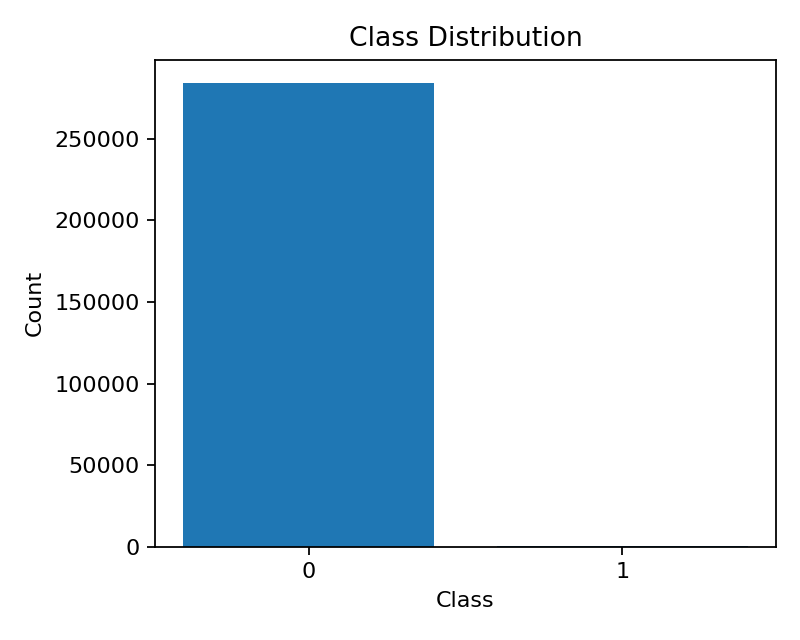
\includegraphics[width=0.75\linewidth]{../artifacts/figures/class_distribution.png}
  \caption{Class distribution (fraud vs non-fraud). Source: \code{artifacts/figures/class_distribution.png}}
\end{figure}

\begin{figure}[H]
  \centering
  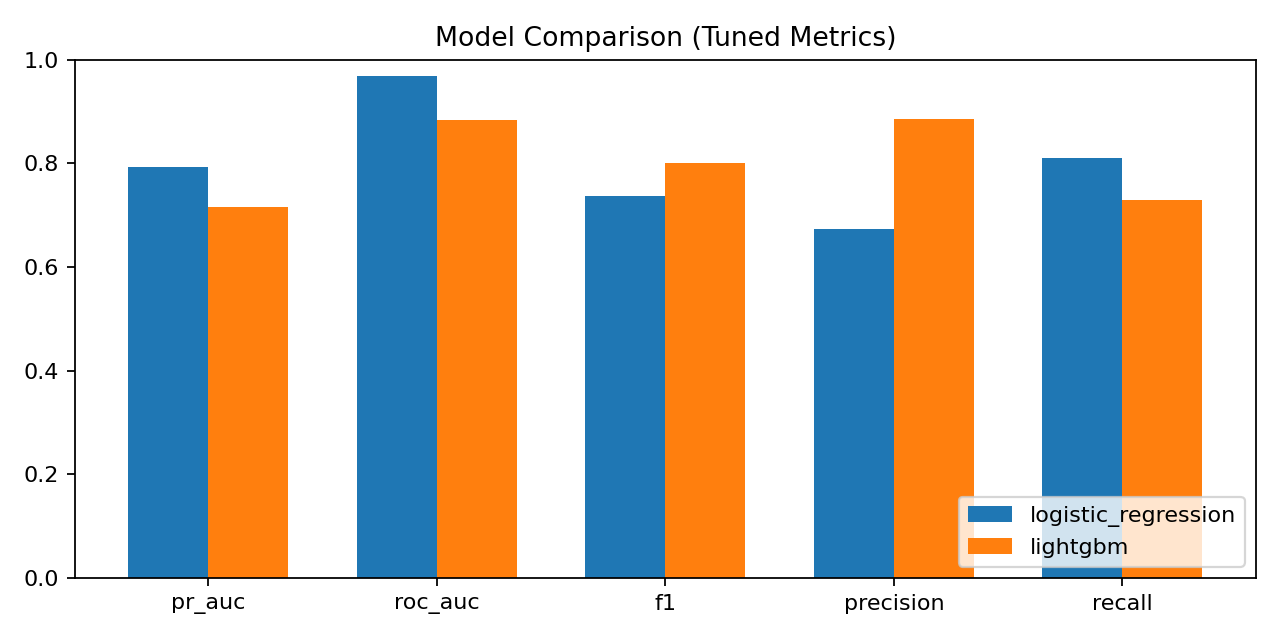
\includegraphics[width=0.85\linewidth]{../artifacts/figures/model_comparison.png}
  \caption{Model comparison of tuned metrics. Source: \code{artifacts/figures/model_comparison.png}}
\end{figure}

\begin{figure}[H]
  \centering
  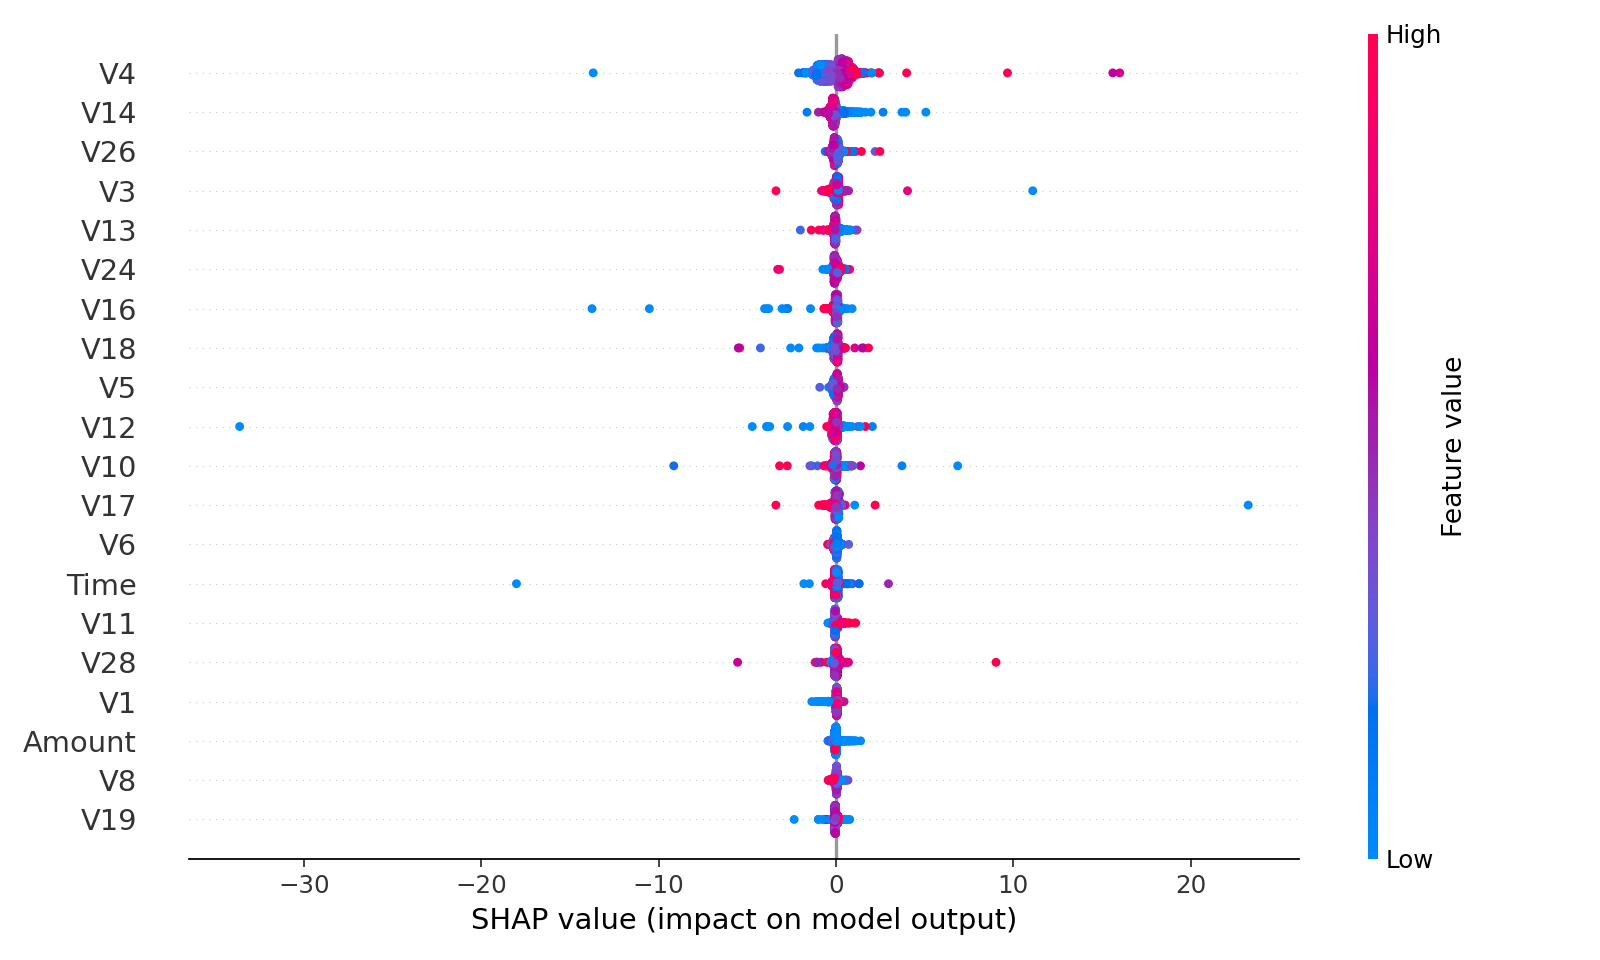
\includegraphics[width=0.9\linewidth]{../artifacts/figures/shap_summary.png}
  \caption{SHAP summary plot (LightGBM explainability). Source: \code{artifacts/figures/shap_summary.png}}
\end{figure}

\end{document}
